% Created 2019-05-09 Thu 15:57
% Intended LaTeX compiler: xelatex
\documentclass[11pt]{article}
\usepackage{graphicx}
\usepackage{grffile}
\usepackage{longtable}
\usepackage{wrapfig}
\usepackage{rotating}
\usepackage[normalem]{ulem}
\usepackage{amsmath}
\usepackage{textcomp}
\usepackage{amssymb}
\usepackage{capt-of}
\usepackage{hyperref}
\usepackage[table]{xcolor}
\usepackage{parskip}
\usepackage[margin=0.3in]{geometry}
\author{Jeremy Barisch-Rooney}
\date{\today}
\title{Timeline of Thesis}
\hypersetup{
 pdfauthor={Jeremy Barisch-Rooney},
 pdftitle={Timeline of Thesis},
 pdfkeywords={},
 pdfsubject={},
 pdfcreator={Emacs 26.2 (Org mode 9.2.3)}, 
 pdflang={English}}
\begin{document}

\maketitle

\section{Overview}
\label{sec:orgc874085}
My goal is to submit the thesis by end of January 2020, and no later.

This will be 8 months of full-time work over a 10 month period. The difference
of two months is because I am initially working part-time on the thesis and
will also take some time off, in particular early on before I leave Amsterdam.

Overleaf you will find a table of weekly work rate and notes/goals of what is
happening per week. You will also find a graph of the work rate.

\pagebreak
\section{Table}
\label{sec:orgd92ccba}
WP = weeks passed, WW = weeks worked

\begin{center}
\label{weekly}
\begin{tabular}{lrrrl}
Date & WP & Rate & WW & Goal/Note\\
\hline
Apr 1 & 1 & 0.5 & 0.5 & Reading\\
Apr 8 & 2 & 0.5 & 1.0 & Research question formulated\\
Apr 15 & 3 & 0 & 1.0 & \cellcolor{blue!25} Time off (catching up on work)\\
Apr 22 & 4 & 0.5 & 1.5 & First draft of abstract and timeline\\
Apr 29 & 5 & 0.5 & 2.0 & Investigated bridge damage types and small scale FE model\\
May 6 & 6 & 0.5 & 2.5 & Project presented to TNO staff\\
May 13 & 7 & 0 & 2.5 & \cellcolor{blue!25} Birthday and father visit\\
May 20 & 8 & 0 & 2.5 & \cellcolor{blue!25} Exam\\
May 27 & 9 & 0.5 & 3.0 & Generated synthetic data under normal conditions\\
Jun 3 & 10 & 1 & 4.0 & Completed literature review\\
Jun 10 & 11 & 0.5 & 4.5 & \cellcolor{blue!25} Mother visit\\
Jun 17 & 12 & 1 & 5.5 & Verified synthetic data against sensor measurements\\
Jun 24 & 13 & 1 & 6.5 & Determined sensors containing explanatory information per damage type\\
July 1 & 14 & 1 & 7.5 & \\
Jul 7 & 15 & 1 & 8.5 & \\
Jul 14 & 16 & 1 & 9.5 & Determined optimal sensor placement for bridge 705\\
Jul 21 & 17 & 0 & 9.5 & \cellcolor{blue!25} Time off\\
Jul 28 & 18 & 0 & 9.5 & \cellcolor{blue!25} Time off and move closer to the office\\
Aug 5 & 19 & 1 & 10.5 & \\
Aug 12 & 20 & 1 & 11.5 & \\
Aug 19 & 21 & 1 & 12.5 & Calculated damage to bridge 705 with a data-driven model\\
Aug 26 & 22 & 1 & 13.5 & \\
Sep 2 & 23 & 1 & 14.5 & Calculated damage to bridge 705 with a finite element model\\
Sep 9 & 24 & 1 & 15.5 & Determined useful combinations of data-driven and finite element models\\
Sep 16 & 25 & 1 & 16.5 & \\
Sep 23 & 26 & 1 & 17.5 & \\
Sep 30 & 27 & 1 & 18.5 & Quantified measurement and model uncertainty\\
Oct 7 & 28 & 1 & 19.5 & Outlined a decision support system\\
Oct 14 & 29 & 1 & 20.5 & Completed a cost-beneft analysis of the decision support system\\
Oct 21 & 30 & 1 & 21.5 & Started generalizing the model to bridges other than 705\\
Oct 28 & 31 & 1 & 22.5 & \\
Nov 4 & 32 & 1 & 23.5 & \\
Nov 11 & 33 & 1 & 24.5 & \\
Nov 18 & 34 & 1 & 25.5 & Started writing thesis\\
Nov 25 & 35 & 1 & 26.5 & \\
Dec 2 & 36 & 1 & 27.5 & \\
Dec 9 & 37 & 1 & 28.5 & Finished writing draft of thesis\\
Dec 16 & 38 & 1 & 29.5 & \\
Dec 23 & 39 & 0 & 29.5 & \cellcolor{blue!25} Time off\\
Dec 30 & 40 & 0 & 29.5 & \cellcolor{blue!25} Time off\\
Jan 6 & 41 & 1 & 30.5 & \\
Jan 13 & 42 & 1 & 31.5 & \\
Jan 20 & 43 & 1 & 32.5 & \\
Jan 27 & 44 & 1 & 33.5 & Submit\\
\end{tabular}
\end{center}

\section{Plot}
\label{sec:orgf4af434}
\begin{center}
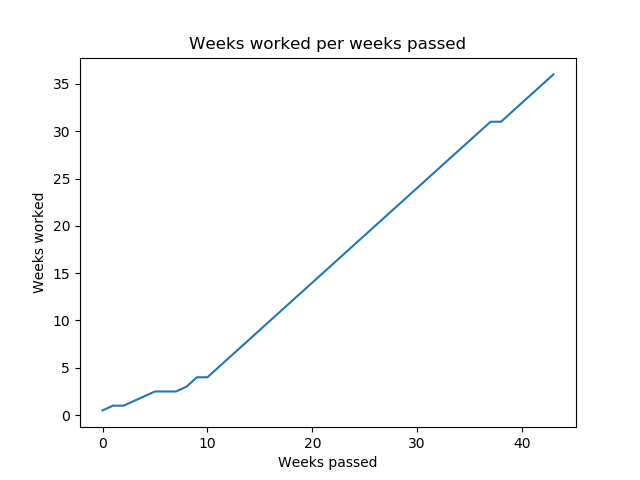
\includegraphics[width=.9\linewidth]{weeks.png}
\end{center}
\end{document}
